\documentclass[a4paper,11pt]{article}

\usepackage[utf8]{inputenc}
\usepackage[francais]{babel}
\usepackage{amsmath}

\usepackage[default]{mathpazo}
\usepackage[T1]{fontenc}

\usepackage{url}
\usepackage{hyperref}
\urlstyle{sf}

\usepackage{titlesec}
\newcommand{\sectionbreak}{\clearpage}

\usepackage{graphicx}
\setkeys{Gin}{width=\textwidth}

\usepackage{setspace}
\setstretch{1.3}
\setlength{\parindent}{0pt}
\baselineskip=30pt
\setlength{\parskip}{\bigskipamount}

% secdot package for adding dot after section numbers
\usepackage{secdot}
\sectiondot{section}
\sectiondot{subsection}
\sectiondot{subsubsection}

% prevent overfull lines
\sloppy

% mdinlinecode command for including code snippets inline
% (fake verbatim, so all special character should be escaped,
% or textmode equivalents of special characters should be used)
\newcommand{\mdinlinecode}[1]{%
    \begin{tikzpicture}[baseline=0ex]%
        \node[anchor=base,%
            text height=1em,%
            text depth=1ex,%
            inner ysep=0pt,%
            draw=mdinlinecodeboxframecolor,%
            fill=mdinlinecodeboxbackgroundcolor,%
            rounded corners=2pt] at (0,0) {\footnotesize\texttt{#1}};%
    \end{tikzpicture}%
}

\title{Microcorruption.com Write-up}
\author{David Wong}
\date{7 Décembre 2014}

\begin{document}

\maketitle


\section{Level 1: Tutorial}\label{level-1-tutorial}

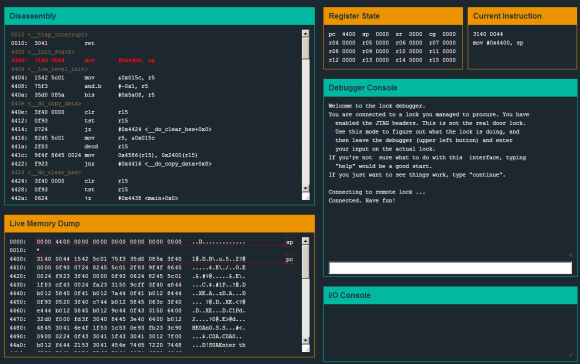
\includegraphics{img/1_1.png}

\href{http://microcorruption.com/}{MicroCorruption} is a ``game'' made
by \textbf{Matasano} in which you will have to debug some programs in
\textbf{assembly}. There is a total of 19 levels and they get harder and
harder, teaching you about more advanced attacks and ways of mitigating
them. The first levels are easy and there is even a tutorial that takes
you step by step into this world. It is a great tool to learn and I
would even say a great game to play. As I had never done any
\textbf{asm} (assembly) prior to this, I will try to document my journey
in this challenge.

\section{Level 2: New Orleans}\label{level-2-new-orleans}

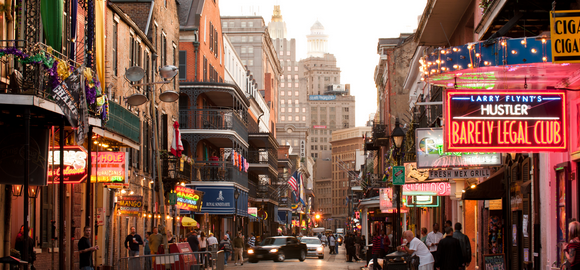
\includegraphics{img/2_3.png}

MicroCorruption comes with a nice debugger. Writing \texttt{c} (as
\emph{continue}) in the \textbf{debugger console} runs the program and
allows you to try a password.

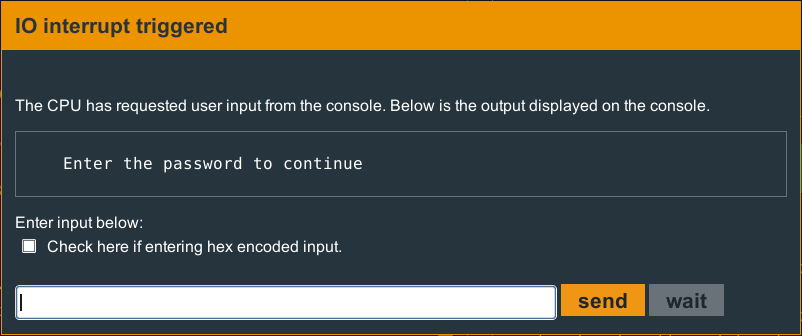
\includegraphics{img/1_2.png}

Of course entering \emph{password} as password doesn't work. let's type
\texttt{reset} in the console and try again. The debugger creates a
\textbf{breaking point} automatically after the pop-up by the way.

After a few \texttt{n} (next instruction) we end up in a
\texttt{check\_password} function. Obviously it is checking if the
password is correct. This is where it starts.

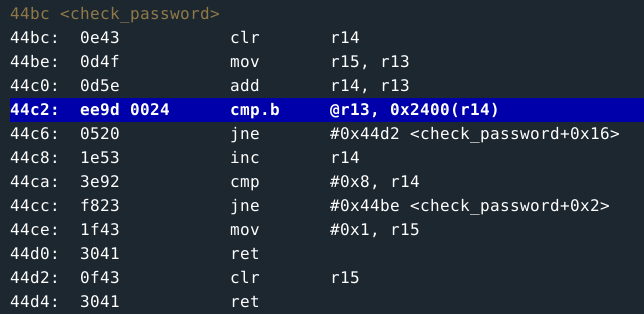
\includegraphics{img/1_3.png}

Some explanations on the desassembly here:

\begin{itemize}
\item
  On the left you can see the addresses in the memory for each
  instructions. They take 16 bits of space (so we are not in a 32 or 64
  bits system) and they are written in base 16 for more conveniance. 1
  bit in the address maps to 1 byte of code. Also an instruction's size
  can vary from 1 byte to many bytes.
\item
  After the address of the instruction you can see the instruction in
  hexadecimal (\texttt{0e43} on the first line). It's not very useful,
  at least at this level.
\item
  Following the hexadecimal form of the instruction you have the
  assembly form of it. Comprised of an \textbf{opcode} (\texttt{clr} on
  the first line) and its \textbf{arguments} (\texttt{r14} on the first
  line).
\end{itemize}

In the function \texttt{check\_password} the program plays with
registers. Those are just places near the CPU that can be accessed very
fast. You can put \textbf{one word} of anything you want in it, be it a
pointer or a value. A \textbf{word} represents the space in memory you
can allocate. MSP430 is a 16 bits system so a word is 16 bits.

There are other ways (and slower ways) to store and retrieve data in
code execution. But we'll only work with registers for this second level.
Here's what the code would do if disassembled in a language more
familiar (that looks like C):

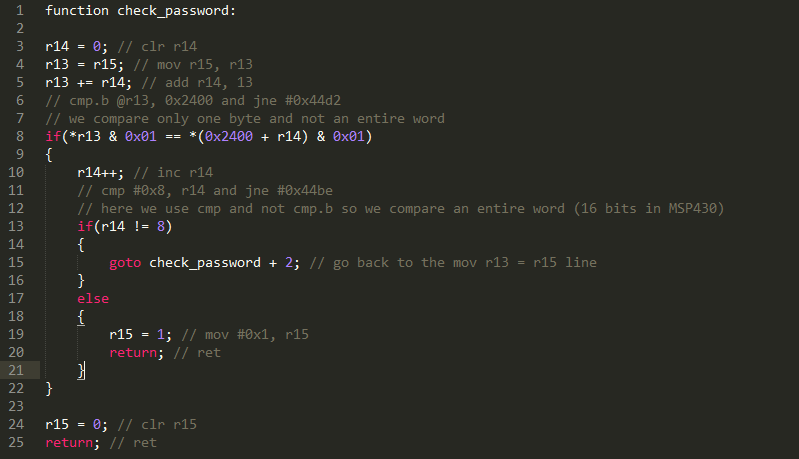
\includegraphics{img/code1_final.PNG}

So we compare one byte of what's in r13 with one byte of what's in
address r14 + 2400 (which is address 2400 since we did a
\texttt{clr r14}).\\Then we compare the next byte, and on and on, for 8
bytes. Then it sets r15 to 1 and return. Otherwise r15 is set to zero.

We can see later in the code that if \texttt{r15 = 0} it's a bad thing,
and if it equals \texttt{1} then we're done!\\At this point we can
easily guess that what is at the address 0x2400 and of length 7 bytes
(followed by the \textbackslash{}0 terminating character) must be the
password.

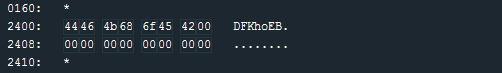
\includegraphics{img/1_6.png}

The live \textbf{memory dump} gives us a string. We enter it as the
password: it works!\\We couldn't see that without running the program
because the password was created during runtime, we can see the function
that does that here:

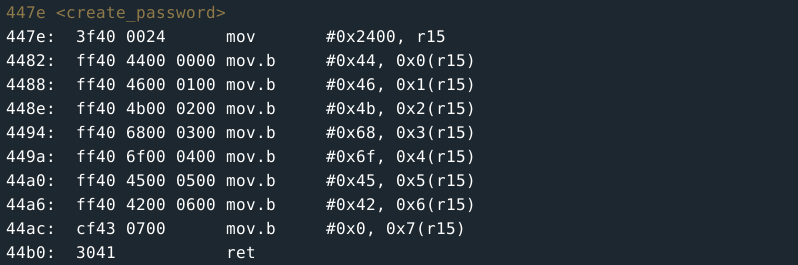
\includegraphics{img/1_5.png}

\section{Level 3: Sydney}\label{level-3-sydney}

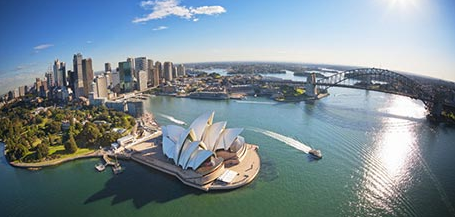
\includegraphics{img/3_2.PNG}

\subsection{Observations}\label{observations}

Let's quickly check the code. We can see that it looks a lot like level
1. We have a \texttt{check\_password} function that has to change
\texttt{r15} to something which is not zero.

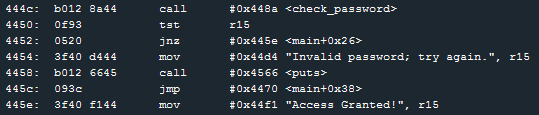
\includegraphics{img/2_1.PNG}

Alright let's look at \texttt{check\_password} shall we?

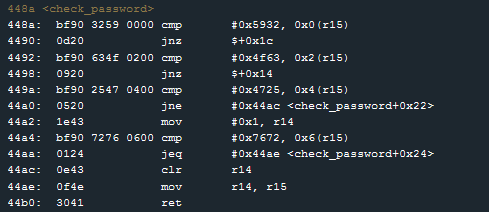
\includegraphics{img/2_2.PNG}

So \texttt{0x5932} (the \texttt{0x} part means we write in hexadecimal!)
is getting compared against r15. Since \textbf{MSP430} is 16 bits,
instructions like \texttt{cmp} compare 16 bits by default.\\Then we
compare \texttt{0x4f63} with \texttt{0x2(r15)} which means the content
at address r15 + 2 bytes.\\And on and on. Bad comparisons at every step
makes the program jumps and set r15 to zero which we don't want.

Note that there are two different jumps here:

\begin{itemize}
\itemsep1pt\parskip0pt\parsep0pt
\item
  Relative jumps: \texttt{jnz \$+0x14} (using the relative instruction
  located at ``current instruction + 0x14'')
\item
  Absolute jumps: \texttt{jne \#0x44ac} (using the absolute address of
  the instruction at ``0x44ac'')
\end{itemize}

Note number 2:

\begin{itemize}
\itemsep1pt\parskip0pt\parsep0pt
\item
  jnz: Jump if not zero. If the previous comparison checks it should
  change some flag to zero and the jnz should not work.
\item
  jne: Jump if not equal. Same principle.
\end{itemize}

At this point we could \textbf{guess} that the password is something
like \texttt{0x59324f6347257672}

Well. Curiously this does not work. After a bit of research, maybe we
are in \href{http://en.wikipedia.org/wiki/Endianness}{little-endian}?

Trying \texttt{0x3259634f25477276} it works!

Basically what the \texttt{cmp} opcode does is slicing the 2 bytes we
feed it in chunks of size 1 byte and ordering them accordingly to our
system's endianness. So here it would be in reverse order.

\section{Level 4: Hanoi}\label{level-4-hanoi}

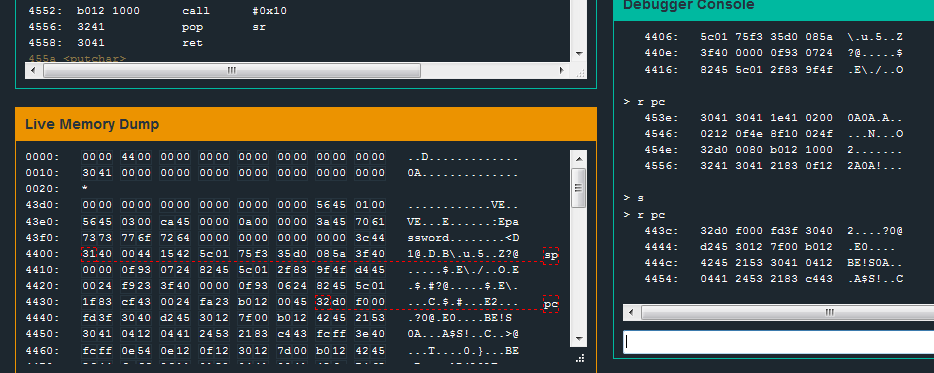
\includegraphics{img/4_1.PNG}

\subsection{Observations}\label{observations-1}

We know how this works now, let's go straight for the \emph{``That
password is not correct.''} line. Scrolling through the {[}code{]} we
can see that a comparison of byte between the value \texttt{0xe0} (224
in decimal) and the content at address \texttt{0x2410}, if it is not
equal the program jumps to address login+0x50. In the Debugger Console
we type \texttt{r login+50} to read the memory at this address. We can
see that it is indeed the line 4570 of the memory which is our
\emph{``That password is not correct.''} line.

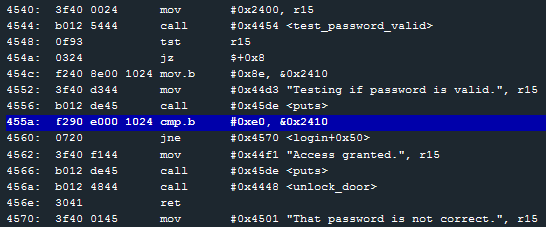
\includegraphics{img/3_1.PNG}

We see that just a few steps ahead, the code sets the byte at
\texttt{0x2410} to \texttt{0x8e}. That is different from \texttt{0xe0}
so the test will inconditionnally fail. Fortunatelly this is avoided if
we jump this instruction. That's exactly what is happening if
\texttt{tst r15} works. Does it?

\begin{itemize}
\itemsep1pt\parskip0pt\parsep0pt
\item
  I set a break point in this instruction with \texttt{b 454a}.
\item
  I run the program with \texttt{c} until it goes to my breakpoint.
\item
  I then \texttt{step} instructions to see that it does makes the jump
  eventhough I entered an incorrect password.
\end{itemize}

So the \texttt{mov.b \#0x8e, \&0x2410} line is just here to confuse us.

\subsection{test\_password\_valid}\label{testux5fpasswordux5fvalid}

Just before calling \texttt{test\_password\_valid} (that seems to be the
function that checks for the correctness of our password) we seem to
move the value \texttt{0x2400} in the \texttt{r15} register. What's
there?

\begin{itemize}
\itemsep1pt\parskip0pt\parsep0pt
\item
  I set a break point in this instruction with \texttt{b 4540}
\item
  I run the program with \texttt{c}
\item
  I enter some dumb value in the password field and I continue to my
  breakpoint
\item
  Once I'm there I check what's in 0x2400 with \texttt{r 2400}, I get
  the dumb value I entered.
\end{itemize}

So \texttt{r15} contains the address where the password I entered is
located. \texttt{2400} is the address where the password is located.

\subsection{what if?}\label{what-if}

What if I entered a password long enough to reach the address
\texttt{2410} so I could put the \texttt{0xe0} value there and my work
would be done?

\begin{quote}
Let's remember. An address contains 1 byte, so we have to write 1 byte
of password to reach the next address. In hexadecimal that's two
letters.
\end{quote}

Let's try to enter \texttt{0xaaaaaaaaaaaaaaaaaaaaaaaaaaaaaaaae0}.
\textbf{It works!}

\section{Level 5: Cusco}\label{level-5-cusco}

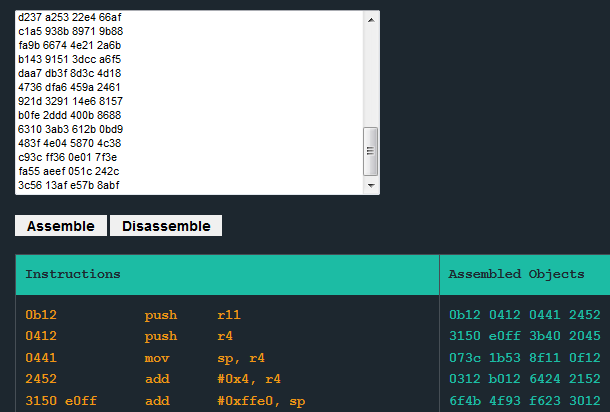
\includegraphics{img/5_1.PNG}

\subsection{Let's start}\label{lets-start}

\begin{quote}
We have fixed issues with passwords which may be too long.
\end{quote}

The message greeting us is quickly confirmed by a test. If we try to
enter a long password it only stores its first 48 bytes in the stack.

We also see that if we run the program with a long password it stops
running correctly after a certain line: the return instruction
\texttt{ret} of the function \texttt{login}. It seems we have overwrote
the instructions. A quick look at the program counter (\texttt{r pc 8})
shows that the next instructions are all zeros.

The \texttt{ret} instruction of a function takes the last value in the
stack and loads it into the Program Counter \texttt{pc}
(\href{http://en.wikipedia.org/wiki/Program_counter}{also called the
Instruction Pointer \texttt{ip} in intel x86}).\\What we did was
overwriting the stack (\textbf{stack overflow}) until it reached what we
call the \textbf{saved pc} of the function (the instruction that is
supposed to run after calling the function).

\subsection{Where is the value we have to
change?}\label{where-is-the-value-we-have-to-change}

Okay, so where exactly is this return value we have to change? I will
enter ``password'' as input so I can quickly find it in the memory. Also
let's add a breakpoint on the \texttt{ret} instruction and see what is
the SP (stack pointer) pointing on.

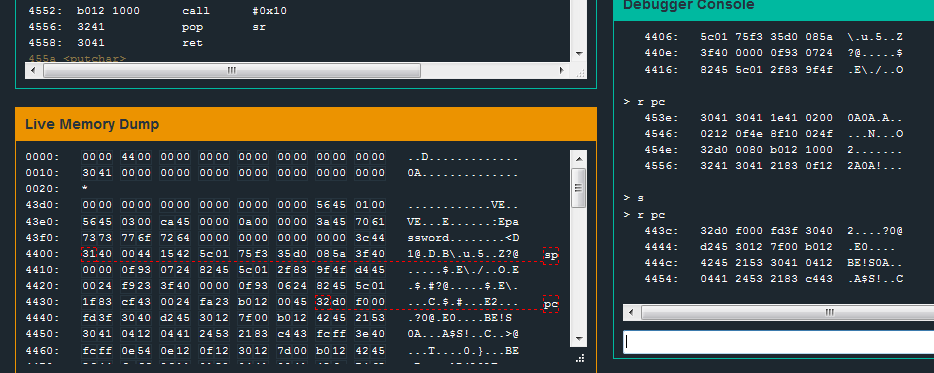
\includegraphics{img/5_2.PNG}

Here we see that \texttt{pc} was pointing to \texttt{453e}, and after
the return it points to address \texttt{443c} in memory, which was
indeed the last 16bits entry of the stack, located 8bytes after our
``password'' (we can see that in the Live Memory Dump). Now we know that
if we enter a password where the 16th byte is 0xaabb, the program will
load the instruction located at address 0xbbaa in memory (remember, we
are in little endian).

\subsection{What should we load?}\label{what-should-we-load}

What about that function called \texttt{unlock\_door}? Let's try to jump
to that and see if it does what it says.

Let's try with that password:
\texttt{0xaaaaaaaaaaaaaaaaaaaaaaaaaaaaaaaa4644}

\textbf{It works!}

\section{Level 6: Reykjavik}\label{level-6-reykjavik}

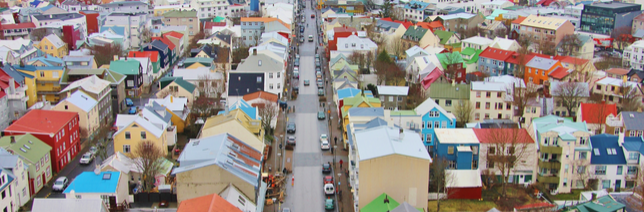
\includegraphics{img/6_1.PNG}

\subsection{Observations}\label{observations-2}

We run the program and hodiho! It seems like at one point our
\texttt{pc} gets lost in the stack and doesn't follow the initial path.

Entering a large number of the same letter we see that they get stored
at address \texttt{43da} in memory.

\subsection{Encryption}\label{encryption}

If you look at the code, you can see that all \texttt{enc} does is
looping and modifying bits of memory. Basically what it does is
\textbf{building instructions} that we will read afterward by
\textbf{pointing the Program Counter on them}. It's mostly
incomprehensible so let's not waste time with this. \texttt{r pc 100}
gives us the hexadecimal code that we can then Disassemble through
Microcorruption Disassembler, or we can just step through it and observe
what is really happening through the Current Instruction window.

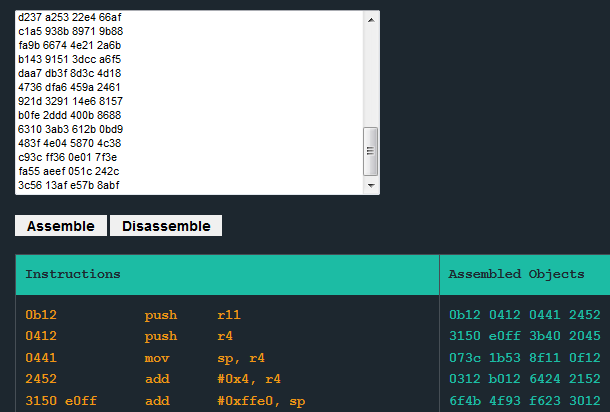
\includegraphics{img/6_3.PNG}

Let's run the code until we get prompted by the pop-up asking for a
password. We can then check that it gets saved into the stack
(\texttt{r sp}). Then let's follow the code step by step with
\texttt{s}. The PC is now following instructions in the stack (which is
normally not possible if the system is protected with the NX bit which
prevents the heap and the stack to be executed).

Right after the popup, this code appears:

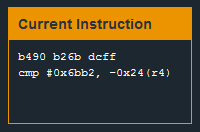
\includegraphics{img/6_2.PNG}

The instruction compares \texttt{0x6bb2} with what is at the address
pointed by \texttt{r4}, minus 24 bytes. Magically, this is where our
password is stored. Remember, \textbf{the instruction \texttt{cmp}
compares 16bits in MSP430}, so the password starts like this:
\texttt{0xb26b} (remember we are in \textbf{little endian}!). Stepping
through the code we don't see anymore \texttt{cmp}. Let's try this value
as a password. \textbf{It works!}

\section{Level 7: Whitehorse}\label{level-7-whitehorse}

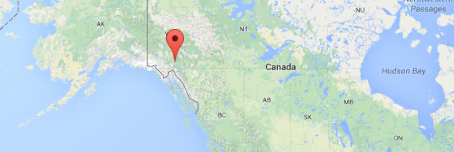
\includegraphics{img/7_1.PNG}

\subsection{Observations}\label{observations-3}

We quickly test our program and see that we can enter a password of
maximum 48 bytes and that we have a \textbf{stack overflow} after a
length of 16 bytes.

The Program jumps to the address located in the bytes number 17 and 18
of our password, this occurs after the Interrupt that checks our
password.

\subsection{Where should we jump?}\label{where-should-we-jump}

The program uses \textbf{HSM-2} to check the password. We don't have
access to it. In the \textbf{LockIT Pro Manual} we can read:

\begin{quote}
\textbf{INT 0x7F.}\\Interface with deadbolt to trigger an unlock if the
password is correct.\\Takes no arguments
\end{quote}

We just have to call a \textbf{0x7F interrupt}. To tell that to the
program we have to simulate the \texttt{push \#0x7F} so that the
interrupt would work.

If we enter this password:
\texttt{aaaaaaaaaaaaaaaaaaaaaaaaaaaaaaaa60447f}

When the \texttt{ret} will occurs, it will set the Program Counter to
\texttt{4460} (where the Stack Pointer is). Then the SP will move to the
value \texttt{7f} which will be taken as an argument when the interrupt
will happen. That's exactly what we want, and it works.

\section{Level 8: Montevideo}\label{level-8-montevideo}

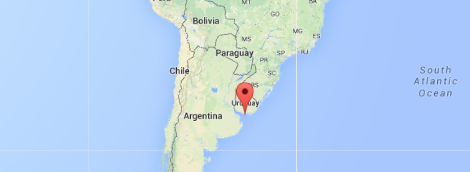
\includegraphics{img/8_1.PNG}

\subsection{Observations}\label{observations-4}

We can enter a 3x16bytes password (same as previous level).\\The program
uses strcpy and memset (this is new).\\We have a stack overflow after 16
bytes (like the previous level).\\So let's try entering the exact same
password \emph{aaaaaaaaaaaaaaaaaaaaaaaaaaaaaaaa60447f}.

It works\ldots{}

(I think it comes from the use of strcpy, it copies until it finds a
\textbackslash{}0 but we can still overflow the stack, buffer overflow,
particularly a stack overflow. This is stack smashing because we change
the RIP (return instruction pointer) here maybe it would be called RPC
(return program counter?))

(The function copies a supplied string without bounds checking by\\using
strcpy() instead of strncpy().
(\url{http://insecure.org/stf/smashstack.html}))

\section{Level 9: Johannesburg}\label{level-9-johannesburg}

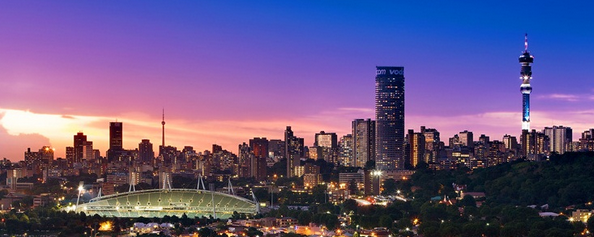
\includegraphics{img/9_2.PNG}

\subsection{Quick Look}\label{quick-look}

There is now a security against passwords that exceed a certain number
of letters, but the security happens after storing it in stack so we can
still store a longer password than expected. The maximum possible seems
to be 37bytes. But the last \texttt{ret} is avoided by a \texttt{br}
(branch to destination) and the program is shut down early, so no stack
overflow here.

\subsection{How is the password's length
checked?}\label{how-is-the-passwords-length-checked}

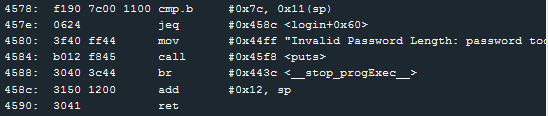
\includegraphics{img/9_1.PNG}

Seems like a password of length superior than 17 bytes is too much, to
test the security of this it just checks if the value located after the
17byte password in the stack is 0x7c, a value that is supposed to be
here.\\\texttt{cmp.b   \#0x7c, 0x11(sp)}

Here's the trick, if we set the 18th byte of our password to 0x7c then
it will work!

We can then jump to the call interrupt and set the last byte of the
stack to 0x7f like we did in the previous levels:

the password \texttt{aaaaaaaaaaaaaaaaaaaaaaaaaaaaaaaaaa7c6c447f} works.

\section{Level 10: Santa Cruz}\label{level-10-santa-cruz}

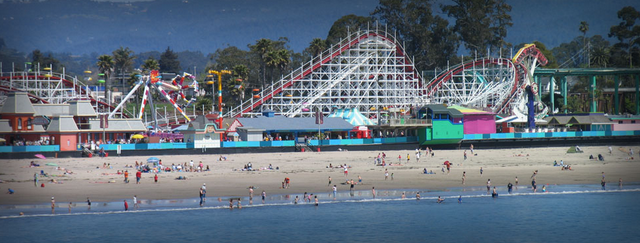
\includegraphics{img/10_5.PNG}

\subsection{First protection}\label{first-protection}

We try entering a long username and password and we get directly kicked
out of the program at line 460c. The program seems to check address
r4-19 (0x43b3) and compare it with r11. If it doesn't match then it
exits.

\textbf{The r11 register seems to hold the password length.}

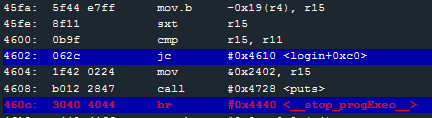
\includegraphics{img/10_1.PNG}

\texttt{jc} Jump on Carry, similar to Jump if Below (\emph{JB}) or Jump
if Not Above or Equal (\texttt{JNAE})

We can circumvent that if what is at address \texttt{0x43b3} is
\textbf{below than the password's length}.

We check this address to see that it's overflowed by the
\textbf{username} we entered. We can set the 18th byte of the username
to something lower than the password length and it will pass the test.

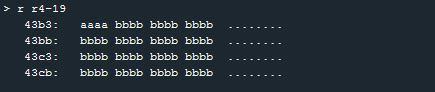
\includegraphics{img/10_2.PNG}

\begin{quote}
here I entered a series of \emph{a}'s as username, and a series of
\emph{b}'s as password.
\end{quote}

\subsection{Second protection}\label{second-protection}

We get kicked a second time but at a different line (45f6).

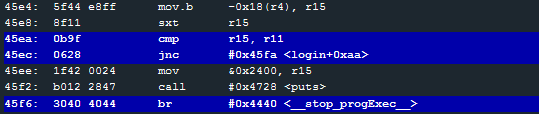
\includegraphics{img/10_3.PNG}

\texttt{jnc} Jump No Carry, equivalent to Jump if Not Below (JNB) or
\textbf{Jump if Above or Equal} (JAE). So we jump if the byte at address
\texttt{0x43b4} \textbf{is not below the password's length}. This
address can be modified by the 19th byte of the username.

\begin{quote}
Note that the initial values are respectively 8 and 10, meaning that
they expected us to enter a password greater than 8 and lesser than 11
characters.
\end{quote}

\subsection{Third protection}\label{third-protection}

We get halted one last time at line 0x465a.

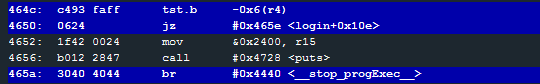
\includegraphics{img/10_4.PNG}

\texttt{tst.b -0x6(r4)}: if the byte at address r4 - 6 (\texttt{0x43c6})
is not zero, it will exit. This is very important as this is one of the
first occurence of a real world way to prevent attacks on a program. It
is called a \textbf{Canary}. It checks for values in the code and detect
buffer overflows if the value is incorrect. Here it checks the byte we
overflowed with the 18th byte of the password we entered.

Thus, this combination of username and password should pass the three
tests we described:

\subsection{Stack Overflow}\label{stack-overflow}

We passed all the test and couldn't produce a stack overflow with the
password. Did I miss something? Let's try with the username

username: aaaaaaaaaaaaaaaaaaaaaaaaaaaaaaaaaa01ffaaa {[}\ldots{}{]}
aaa\\password: bbbbbbbbbbbbbbbbbbbbbbbbbbbbbbbbbb00

That's the solution. The Stack Pointer points to some remains of the
username right before executing the last \texttt{ret} of our program. We
can now do a stack overflow by modyfing the 43th byte of the username to
the address we want to jump to.

We use the 7F call interrupt technique of the previous challenge.

username:
aaaaaaaaaaaaaaaaaaaaaaaaaaaaaaaaaa01ffaaaaaaaaaaaaaaaaaaaaaaaaaaaaaaaaaaaaaaaaaaaaaa72447f\\password:
bbbbbbbbbbbbbbbbbbbbbbbbbbbbbbbbbb00

\textbf{It works!}

\section{Level 11: Jakarta}\label{level-11-jakarta}

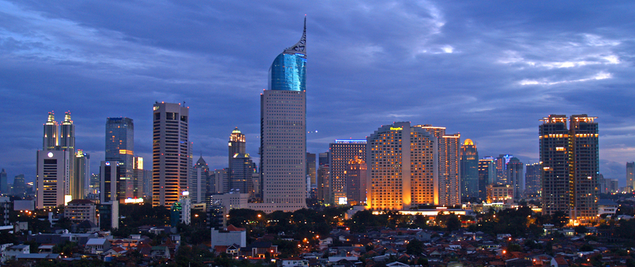
\includegraphics{img/11_6.PNG}

\subsection{First protection}\label{first-protection-1}

Entering different usernames we see that \textbf{r11 is the username's
length}.\\Look at the instruction \texttt{cmp.b \#0x21, r11}

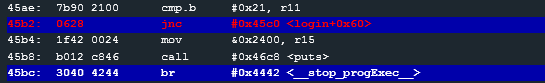
\includegraphics{img/11_1.PNG}

\begin{quote}
\texttt{jnc} \textasciitilde{} Jump if Above or Equal
\end{quote}

So we pass the first test if \textbf{the username's length is lesser
than 33 bytes} (0x21).

\subsection{Second protection}\label{second-protection-1}

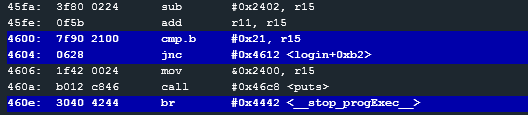
\includegraphics{img/11_2.PNG}

\begin{verbatim}
add r11, r15
cmp.b #0x21, r15
jnc
\end{verbatim}

So \textbf{the sum of the username and the password lenghts} have to be
lesser than 33 bytes as well (0x21).

\subsection{Stack Overflow}\label{stack-overflow-1}

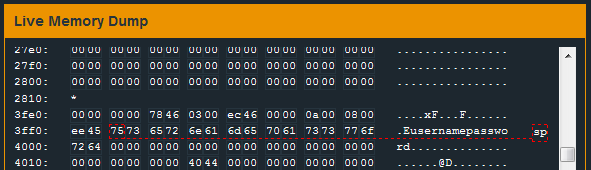
\includegraphics{img/11_3.PNG}

We see that the username and the password are stored in the stack thanks
to the \texttt{strcpy}.

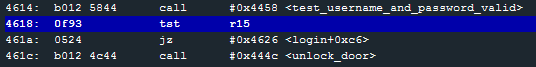
\includegraphics{img/11_4.PNG}

We see that the password is tested in the function
\texttt{test\_username\_and\_password\_valid} through the 7d interrupt.
So we cannot do anything here. It is obvious we need to create a stack
overflow again.

But let's go back to our previous tests

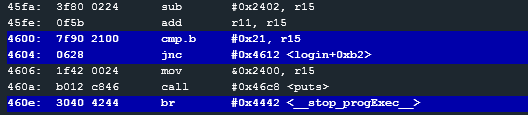
\includegraphics{img/11_2.PNG}

Don't you see something? \texttt{cmp.b \#0x21, r15}.\\This means:
compare byte of r15 and 0x21. But words are 2 bytes in MSP430 (so
registers and address in the stack are 2 bytes).\\What if we wrote
0x1020 for example. Would it be lesser than 0x21 ?

Let's try that.

I enter
\texttt{aaaaaaaaaaaaaaaaaaaaaaaaaaaaaaaaaaaaaaaaaaaaaaaaaaaaaaaaaaaaaaaa}
(length of 0x20) as username.

we want the toal to be 0x0100 to test our hypothesis. So we need 0xd0
more (14 * 16 = 224 bytes).

Entering
\texttt{bbbbbbbbbbbbbbbbbbbbbbbbbbbbbbbbbbbbbbbbbbbbbbbbbbbbbbbbbbbbbbbbbbbbbbbbbbbbbbbbbbbbbbbbbbbbbbbbbbbbbbbbbbbbbbbbbbbbbbbbbbbbbbbbbbbbbbbbbbbbbbbbbbbbbbbbbbbbbbbbbbbbbbbbbbbbbbbbbbbbbbbbbbbbbbbbbbbbbbbbbbbbbbbbbbbbbbbbbbbbbbbbbbbbbbbbbbbbbbbbbbbbbbbbbbbbbbbbbbbbbbbbbbbbbbbbbbbbbbbbbbbbbbbbbbbbbbbbbbbbbbbbbbbbbbbbbbbbbbbbbbbbbbbbbbbbbbbbbbbbbbbbbbbbbbbbbbbbbbbbbbbbbbbbbbbbbbbbbbbbbbbbbbbbbbbbbbbbbbbbbbbbbbbbbbbbbbbbbbbbbbbbbbbbbbbbbbbbbbbbbbbbbbbb}
it works and we get lost at a random address. We've successfully
overwrote the return address.

Breaking on the return instruction we can see at what address the Saved
PC is (at the SP address).

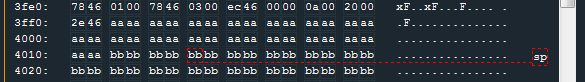
\includegraphics{img/11_5.PNG}

So we can enter our personalized return address at the byte number 5 and
6 of our password (if our username is of length 0x20 of course). Let's
return at the instruction \texttt{unlock\_door}.

So entering the same username, and this as password works:

\texttt{bbbbbbbb1c46bbbbbbbbbbbbbbbbbbbbbbbbbbbbbbbbbbbbbbbbbbbbbbbbbbbbbbbbbbbbbbbbbbbbbbbbbbbbbbbbbbbbbbbbbbbbbbbbbbbbbbbbbbbbbbbbbbbbbbbbbbbbbbbbbbbbbbbbbbbbbbbbbbbbbbbbbbbbbbbbbbbbbbbbbbbbbbbbbbbbbbbbbbbbbbbbbbbbbbbbbbbbbbbbbbbbbbbbbbbbbbbbbbbbbbbbbbbbbbbbbbbbbbbbbbbbbbbbbbbbbbbbbbbbbbbbbbbbbbbbbbbbbbbbbbbbbbbbbbbbbbbbbbbbbbbbbbbbbbbbbbbbbbbbbbbbbbbbbbbbbbbbbbbbbbbbbbbbbbbbbbbbbbbbbbbbbbbbbbbbbbbbbbbbbbbbbbbbbbbbbbbbbbbbbbbbbbbbbbbbbbbbbbbbbbbbbbbb}

\section{Level 12: Addis Ababa}\label{level-12-addis-ababa}

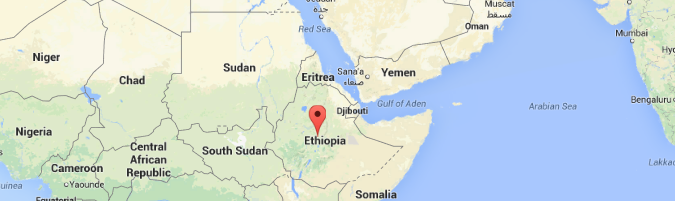
\includegraphics{img/12_1.PNG}

\subsection{Quick observations}\label{quick-observations}

\begin{itemize}
\itemsep1pt\parskip0pt\parsep0pt
\item
  The password is tested through \texttt{test\_password\_valid} with a
  7d interrupt (HSM Model 1).
\item
  We have an \texttt{unlock\_door} function (so no need to go through
  the \texttt{test\_password\_valid} function if we can return to
  it).(44da)
\item
  We have no \texttt{ret} after the main (so we can't modify the return
  address).
\item
  If the SP is different from zero the program unlocks the doors.
\item
  We have a printf of our username (\textbf{format string
  vulnerability}!)
\end{itemize}

\subsection{Printf in Manual}\label{printf-in-manual}

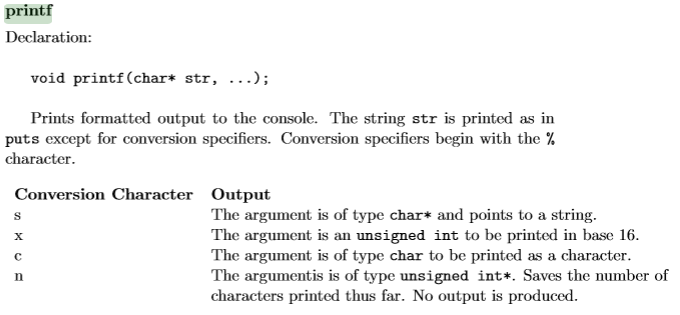
\includegraphics{img/12_2.PNG}

We see that printf is a limited version of the C equivalent. Since we
have \%n available we know we can write to the memory and thus we should
be able to do a Format String exploit.

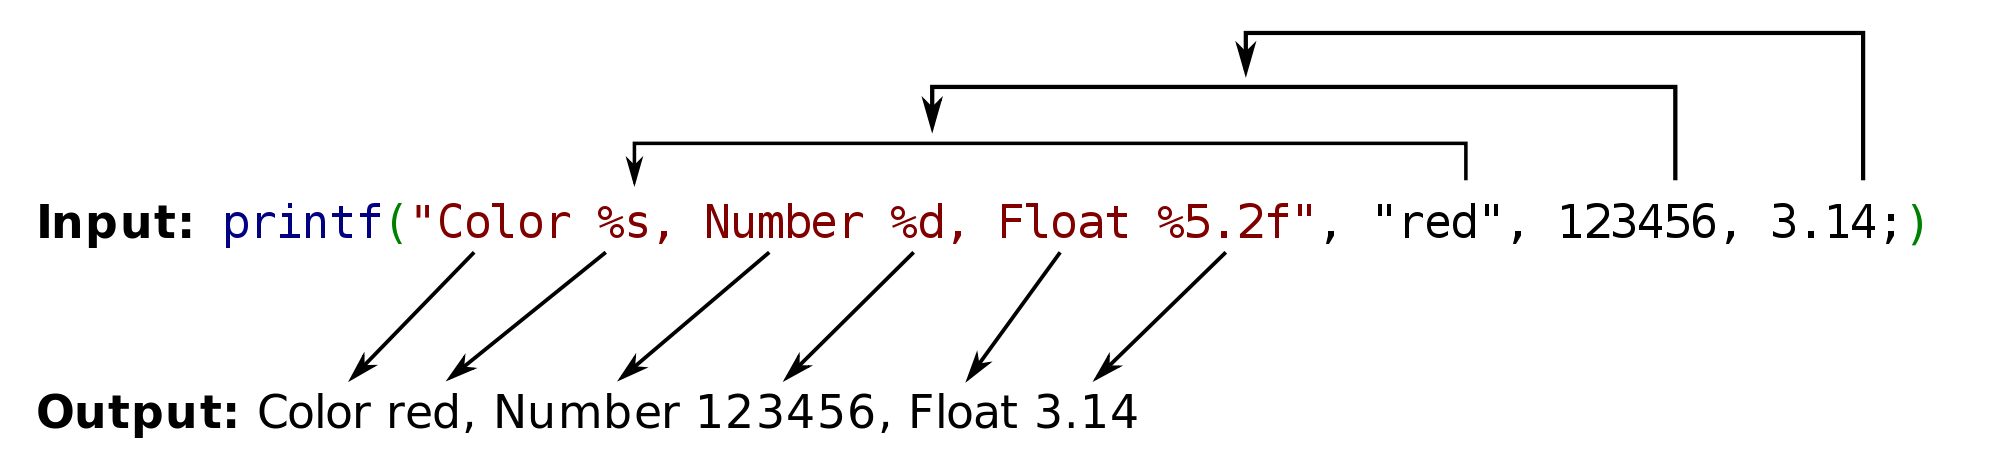
\includegraphics{img/12_3.PNG}

So here the developer did a:

\texttt{printf(user\_input);}

instead of this:

\texttt{printf("\%s", user\_input);}

So the user\_input becomes the format string and it will look in the
stack for its arguments (in the example red, 123456, and \ldots{} are
pushed in the stack).

\subsection{Printf in MSP430}\label{printf-in-msp430}

Let's try \texttt{\%x} as input. It doesn't output anything. So the
first argument must be null:

\texttt{printf(user\_input, 0x00);}

Let's try again with \texttt{\%x \%x}. It outputs \texttt{7825} which is
\texttt{\%x} reversed (little endian). It seems like when we point to
our second arguments we are pointing to the beginning of our input.
Since a word is 16bits in MSP430 we only display 2 characters in
hexadecimal.

So if we enter \texttt{PTR\%x\%n} we will write 5 to the address in
PTR.\\note that we can use \%x, \%c, \%n\ldots{} as our first format
since we won't use it.

\subsection{Exploit}\label{exploit}

Remember what we observed at the begginning:

\begin{quote}
If the SP is different from zero the program unlocks the doors.
\end{quote}

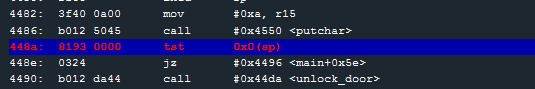
\includegraphics{img/12_5.PNG}

It was at this line. And by breaking on it we can see that sp is
pointing to 3062.

So let's try to do \texttt{6230256e256e}

which should write the number of characters printed before the last \%n
(which will be only 2 since the first \%n won't count).

\section{Level 13: Novosibirsk}\label{level-13-novosibirsk}

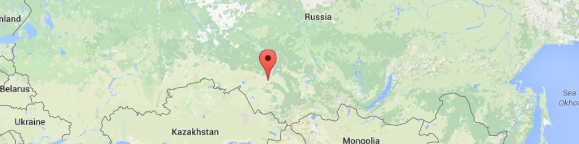
\includegraphics{img/13_1.PNG}

\subsection{Observations}\label{observations-5}

\begin{itemize}
\itemsep1pt\parskip0pt\parsep0pt
\item
  Printf again, except this time the first argument is the user input (a
  simple \texttt{\%x} returns \texttt{7825})
\item
  No main ret.
\item
  Call to \texttt{conditional\_unlock\_door} (HSM-2)
\end{itemize}

\subsection{Format String Again}\label{format-string-again}

The obvious idea here is to change the 7E interrupt to a 7F interrupt.
Let's try the to exploit the Format String to do that.

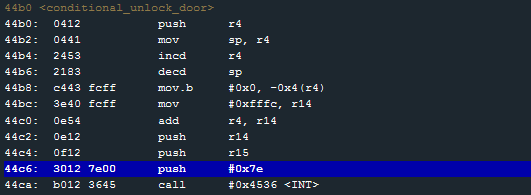
\includegraphics{img/13_2.PNG}

So let's build our input:

\begin{itemize}
\itemsep1pt\parskip0pt\parsep0pt
\item
  the address we want to write on (here \texttt{c844} (little endian)).
\item
  Then enough padding to print 7f (127) bytes including the 4 bytes of
  the address we're writing on.
\item
  The format \%n
\end{itemize}

\texttt{c8446161616161616161616161616161616161616161616161616161616161616161616161616161616161616161616161616161616161616161616161616161616161616161616161616161616161616161616161616161616161616161616161616161616161616161616161616161616161616161616161616161616161256e}

This works.

\section{Level 14: Algiers}\label{level-14-algiers}

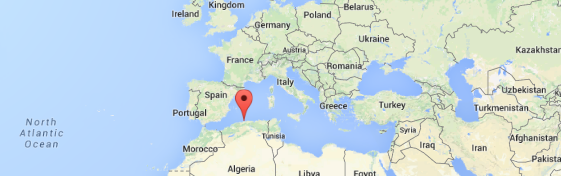
\includegraphics{img/14_1.PNG}

\subsection{Observations}\label{observations-6}

\begin{itemize}
\itemsep1pt\parskip0pt\parsep0pt
\item
  Use of the \textbf{malloc} function. Hints at a \textbf{Heap Overflow
  Exploit}.
\item
  There are two functions that can unlock this level:
  \texttt{unlock\_door} and \texttt{test\_password\_valid}.
\item
  There seem to be no check on the username and password length. We can
  enter 18 bytes in username and then it gets overwritten by password.
\item
  With a quick test entering a long string of the same letter as
  username and as password we get an error : \textbf{load address
  unaligned: UU75} where UU is the character we entered in the username.
\item
  One character in username input gets changed to ` during the password
  verification (at address 2422 in memory).
\item
  The buffer overflow stops us at line 0x4520 (in the \texttt{free}
  function).
\end{itemize}

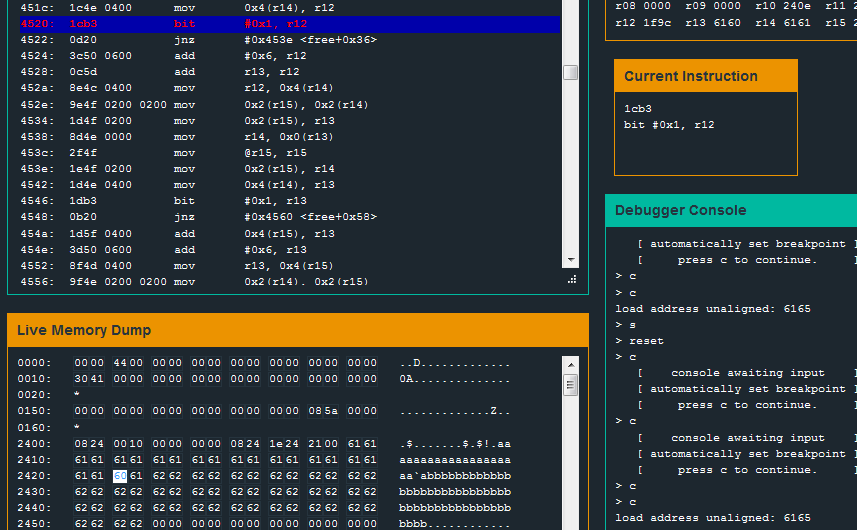
\includegraphics{img/14_2.PNG}

In the Manual we find:

\begin{quote}
BIT arg1 arg2 -\textgreater{} compute arg1 \& arg1, set the flags, and
discard the results (like TEST on x86)
\end{quote}

Also it seems good to keep being aware that in MSP430 the Heap grows
toward the Stack and the Stack towards the Heap.

0000 low addresses\\HEAP v

STACK \^{}\\Text v\\ffff high addresses

\subsection{login}\label{login}

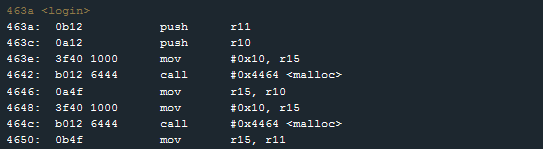
\includegraphics{img/14_3.PNG}

Looking at the login function we see that it's doing two malloc of size
10 and is storing the username in the first malloc contained at r10, and
the password in the second malloc r11.

After retrieving the user's credentials and storing them in the heap.
The program calls \texttt{test\_password\_valid} and unlocks the door or
not according to the validity of the username and the password.

Looking at the test\_password\_valid we see an early \texttt{ret}
followed by a long list of what seems like gibberish opcodes.

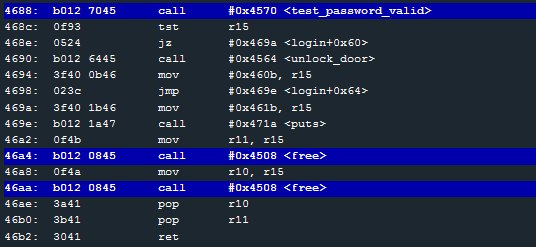
\includegraphics{img/14_4.PNG}

Later the login function frees the two mallocs.

But let's see what really happens. We can see the heap before the
mallocs:

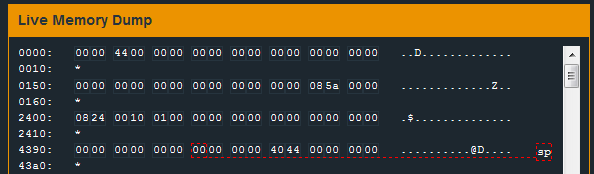
\includegraphics{img/14_5.PNG}

The heap after the first malloc:

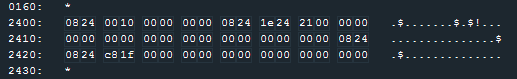
\includegraphics{img/14_6.PNG}

The heap after the second malloc:

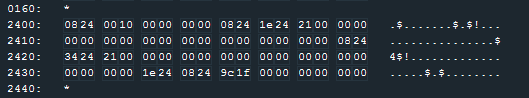
\includegraphics{img/14_7.PNG}

The heap after entering ``username'' as username:

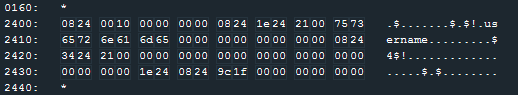
\includegraphics{img/14_8.PNG}

The heap after entering ``password'' as password:

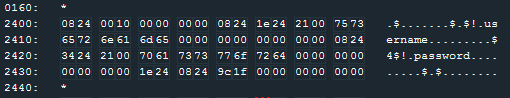
\includegraphics{img/14_9.PNG}

Here we can see the memory after the first free:

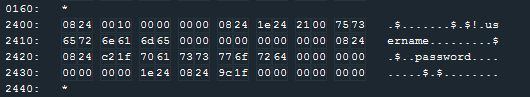
\includegraphics{img/14_10.PNG}

And the memory after the second free:

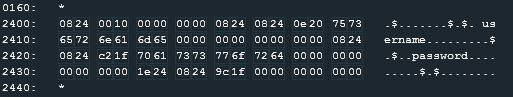
\includegraphics{img/14_11.PNG}

\subsection{Heap Structure.}\label{heap-structure.}

\includegraphics{img/14_9.PNG}

The Heap is a \textbf{doubly-linked list}. Each chunk is composed of
\textbf{metadatas} and a \textbf{payload}. The chunks are wraped with a
heap header and a heap footer. Here we can see the structure of a
chunck:

\begin{verbatim}
0824 | 1e24 | 21 00 | username | 00...
 bk  |  fw  | flag  | payload  | padding
\end{verbatim}

And what is interesting:

\begin{itemize}
\itemsep1pt\parskip0pt\parsep0pt
\item
  bk (backward): a pointer to the previous chunck
\item
  fw (forward): a pointer to the next chunck
\end{itemize}

The second chunck starts at address \texttt{241e} and contains the
password. The idea of a heap overflow is to \textbf{overwrite the
metadatas} of this second chunck when filling the payload of the first
one. Because when free is called to remove this chunck, it will do some
magic with the fw and bk pointers so the chain can reconstruct around
the chunck.

\subsection{Try to exploit this}\label{try-to-exploit-this}

So let's change overwrite the second chunck with our username input. I
tried multipled things:

\begin{itemize}
\itemsep1pt\parskip0pt\parsep0pt
\item
  Set fw to the saved pc in the stack right before the return of the
  login function, set bk to the address where login calls unlock\_door.
\item
  Set fw to the address being called in the second free, set bw to the
  unlock\_door function.
\item
  Set fw to the instruction return in the free function, set bw to Nops
  so we would go directly in the unlock\_door function afterwards.
\end{itemize}

It failed for different reasons. It was overwritting things at the bw
pointer. It was not working because of parity problems. Reversing the
function did help understand that what we would point with fw would
influence the overwriting.

Here is a smart reverse of the function \texttt{free}. It was thought so
I could see how changing bk, fw and the flag would influence the free.
So this is not exactly what the free function does! I also remove
useless lines.

\includegraphics{img/code2_final.PNG}

In the end I tried to make a shell code. I copied the instructions in
unlock\_door:

\begin{verbatim}
3012 7f00 b012 b646 fd3f
\end{verbatim}

And I pointed the saved pc to the heap (which is supposed to be
non-executable on a protected system but here it worked!).

Also, to counter the overwritting problem I made a NOP slide. Here's the
solution:

\texttt{909090909090 3012 7f00 b012 b646 fd3f 0e24 9a43}
\end{document}